%% Lab Report for EEET2493_labreport_template.tex
%% V1.0
%% 2019/01/16
%% This is the template for a Lab report following an IEEE paper. Modified by Francisco Tovar after Michael Sheel original document.


%% This is a skeleton file demonstrating the use of IEEEtran.cls
%% (requires IEEEtran.cls version 1.8b or later) with an IEEE
%% journal paper.
%%
%% Support sites:
%% http://www.michaelshell.org/tex/ieeetran/
%% http://www.ctan.org/pkg/ieeetran
%% and
%% http://www.ieee.org/

%%*************************************************************************
%% Legal Notice:
%% This code is offered as-is without any warranty either expressed or
%% implied; without even the implied warranty of MERCHANTABILITY or
%% FITNESS FOR A PARTICULAR PURPOSE! 
%% User assumes all risk.
%% In no event shall the IEEE or any contributor to this code be liable for
%% any damages or losses, including, but not limited to, incidental,
%% consequential, or any other damages, resulting from the use or misuse
%% of any information contained here.
%%
%% All comments are the opinions of their respective authors and are not
%% necessarily endorsed by the IEEE.
%%
%% This work is distributed under the LaTeX Project Public License (LPPL)
%% ( http://www.latex-project.org/ ) version 1.3, and may be freely used,
%% distributed and modified. A copy of the LPPL, version 1.3, is included
%% in the base LaTeX documentation of all distributions of LaTeX released
%% 2003/12/01 or later.
%% Retain all contribution notices and credits.
%% ** Modified files should be clearly indicated as such, including  **
%% ** renaming them and changing author support contact information. **
%%*************************************************************************

\documentclass[journal]{IEEEtran}

% *** CITATION PACKAGES ***
\usepackage[style=ieee]{biblatex} 

% *** MATH PACKAGES ***
\usepackage{amsmath}

% *** PDF, URL AND HYPERLINK PACKAGES ***
\usepackage{url}
% correct bad hyphenation here
\hyphenation{op-tical net-works semi-conduc-tor}
\usepackage{graphicx}  %needed to include png, eps figures
\usepackage{float}  % used to fix location of images i.e.\begin{figure}[H]

%https://tex.stackexchange.com/questions/230828/when-referencing-a-figure-make-text-and-figure-name-clickable
\usepackage[colorlinks]{hyperref}

\usepackage{pdflscape}
\usepackage{multicol}
\usepackage{listings}
\usepackage{color}
\usepackage[dvipsnames]{xcolor}

%https://tex.stackexchange.com/questions/245842/i-am-trying-to-get-the-image-full-screen-and-landscape
\usepackage{graphicx}
\usepackage[a4paper,margin=1in]{geometry}
\usepackage{lscape}
\usepackage{rotating}
\usepackage{pdflscape}

\definecolor{dkgreen}{rgb}{0,0.6,0}
\definecolor{gray}{rgb}{0.5,0.5,0.5}
\definecolor{mauve}{rgb}{0.58,0,0.82}

\lstset{frame=tb,
language=C++,
aboveskip=3mm,
  belowskip=3mm,
  showstringspaces=false,
  columns=flexible,
  basicstyle={\small\ttfamily},
  numbers=none,
  numberstyle=\tiny\color{gray},
  keywordstyle=\color{blue},
  commentstyle=\color{dkgreen},
  stringstyle=\color{mauve},
  breaklines=true,
  breakatwhitespace=true,
  tabsize=3,
  %https://stackoverflow.com/questions/3915709/latex-lstlisting-automatically-recognizing-code-passage
  rangeprefix=//-LaTeX:,
  rangesuffix=;,
  includerangemarker=false,
  columns=spaceflexible,
  %https://tex.stackexchange.com/questions/106770/how-to-add-line-numbers-to-a-program-listing-code
  numbers=left,
  stepnumber=1
}

\lstdefinelanguage{Ini}
{
    basicstyle=\ttfamily\small,
    columns=fullflexible,
    morecomment=[s][\color{mauve}\bfseries]{[}{]},
    morecomment=[l]{\#},
    morecomment=[l]{;},
    commentstyle=\color{gray}\ttfamily,
    morekeywords={},
    otherkeywords={=,:},
    keywordstyle={\color{green}\bfseries}
}

% https://github.com/GothenburgBitFactory/guides/blob/master/20151107_de_openrheinruhr/yaml_syntax_highlighting.tex
%%%%%%%%%%%%%%%%%%%%%%%%%%%%%%%%%%%%%%%%%%%%%%%%%%%%%%
%%%%%%%%%%% YAML syntax highlighting %%%%%%%%%%%%%%%%%

% http://tex.stackexchange.com/questions/152829/how-can-i-highlight-yaml-code-in-a-pretty-way-with-listings

% here is a macro expanding to the name of the language
% (handy if you decide to change it further down the road)
\newcommand\YAMLcolonstyle{\color{red}\mdseries}
\newcommand\YAMLkeystyle{\color{black}\bfseries}
\newcommand\YAMLvaluestyle{\color{blue}\mdseries}

\makeatletter

\newcommand\language@yaml{yaml}

\expandafter\expandafter\expandafter\lstdefinelanguage
\expandafter{\language@yaml}
{
  keywords={true,false,null,y,n},
  keywordstyle=\color{darkgray}\bfseries,
  basicstyle=\YAMLkeystyle,                                 % assuming a key comes first
  sensitive=false,
  comment=[l]{\#},
  morecomment=[s]{/*}{*/},
  commentstyle=\color{purple}\ttfamily,
  stringstyle=\YAMLvaluestyle\ttfamily,
  moredelim=[l][\color{orange}]{\&},
  moredelim=[l][\color{magenta}]{*},
  moredelim=**[il][\YAMLcolonstyle{:}\YAMLvaluestyle]{:},   % switch to value style at :
  morestring=[b]',
  morestring=[b]",
  literate =    {---}{{\ProcessThreeDashes}}3
                {>}{{\textcolor{red}\textgreater}}1     
                {|}{{\textcolor{red}\textbar}}1 
                {\ -\ }{{\mdseries\ -\ }}3,
}

% switch to key style at EOL
\lst@AddToHook{EveryLine}{\ifx\lst@language\language@yaml\YAMLkeystyle\fi}
\makeatother

\newcommand\ProcessThreeDashes{\llap{\color{cyan}\mdseries-{-}-}}

%%%%%%%%%%% YAML syntax highlighting %%%%%%%%%%%%%%%%%
%%%%%%%%%%%%%%%%%%%%%%%%%%%%%%%%%%%%%%%%%%%%%%%%%%%%%%

\begin{document}

% paper title
\title{Arduino Lab 3}

% author names 
\author{Knut Ola Nøsen
}% <-this % stops a space

% The report headers
\markboth{IELET1002 DATATEKNIKK. LAB. REPORT 3, FEBRUARY 2022}%do not delete next lines
{Shell \MakeLowercase{\textit{et al.}}: Bare Demo of IEEEtran.cls for IEEE Journals}

% make the title area
\maketitle

% As a general rule, do not put math, special symbols or citations
% in the abstract or keywords.
\begin{abstract}
    The project explores multitasking by creating a reaction-based game. The goal is to demonstrate how
    the architecture of an Arduino program can be influenced by its lack of proper multithreading.
    The program contains not only parallel operations, but also the use of Serial input for manipulating
    the game state.
\end{abstract}

\begin{IEEEkeywords}
    Arduino, RGB, LED, Random, RAMP, Sequential, Multithreading
\end{IEEEkeywords}

\section{Theory}
% Here we have the typical use of a "W" for an initial drop letter
% and "RITE" in caps to complete the first word.
% You must have at least 2 lines in the paragraph with the drop letter
% (should never be an issue)

\IEEEPARstart{T}{he}
game centers around reaction time. Two players have a button each, and when the center RGB LED switches
from red to green, the first player to press the button gets points based on the players reaction time.
If the LED turns blue instead of green, the player who clicks a button will loose points. If noone clicks,
the game will continue with a new round after 1 second. The game ends when a player reaches a score of 10 points.
After each round is won/lost, a tone will play and leds flash to celebrate the winner or bully the looser.

\section{Methods}
\subsection{Hardware}

\begin{figure}[H]%[!ht]
    \begin {center}
    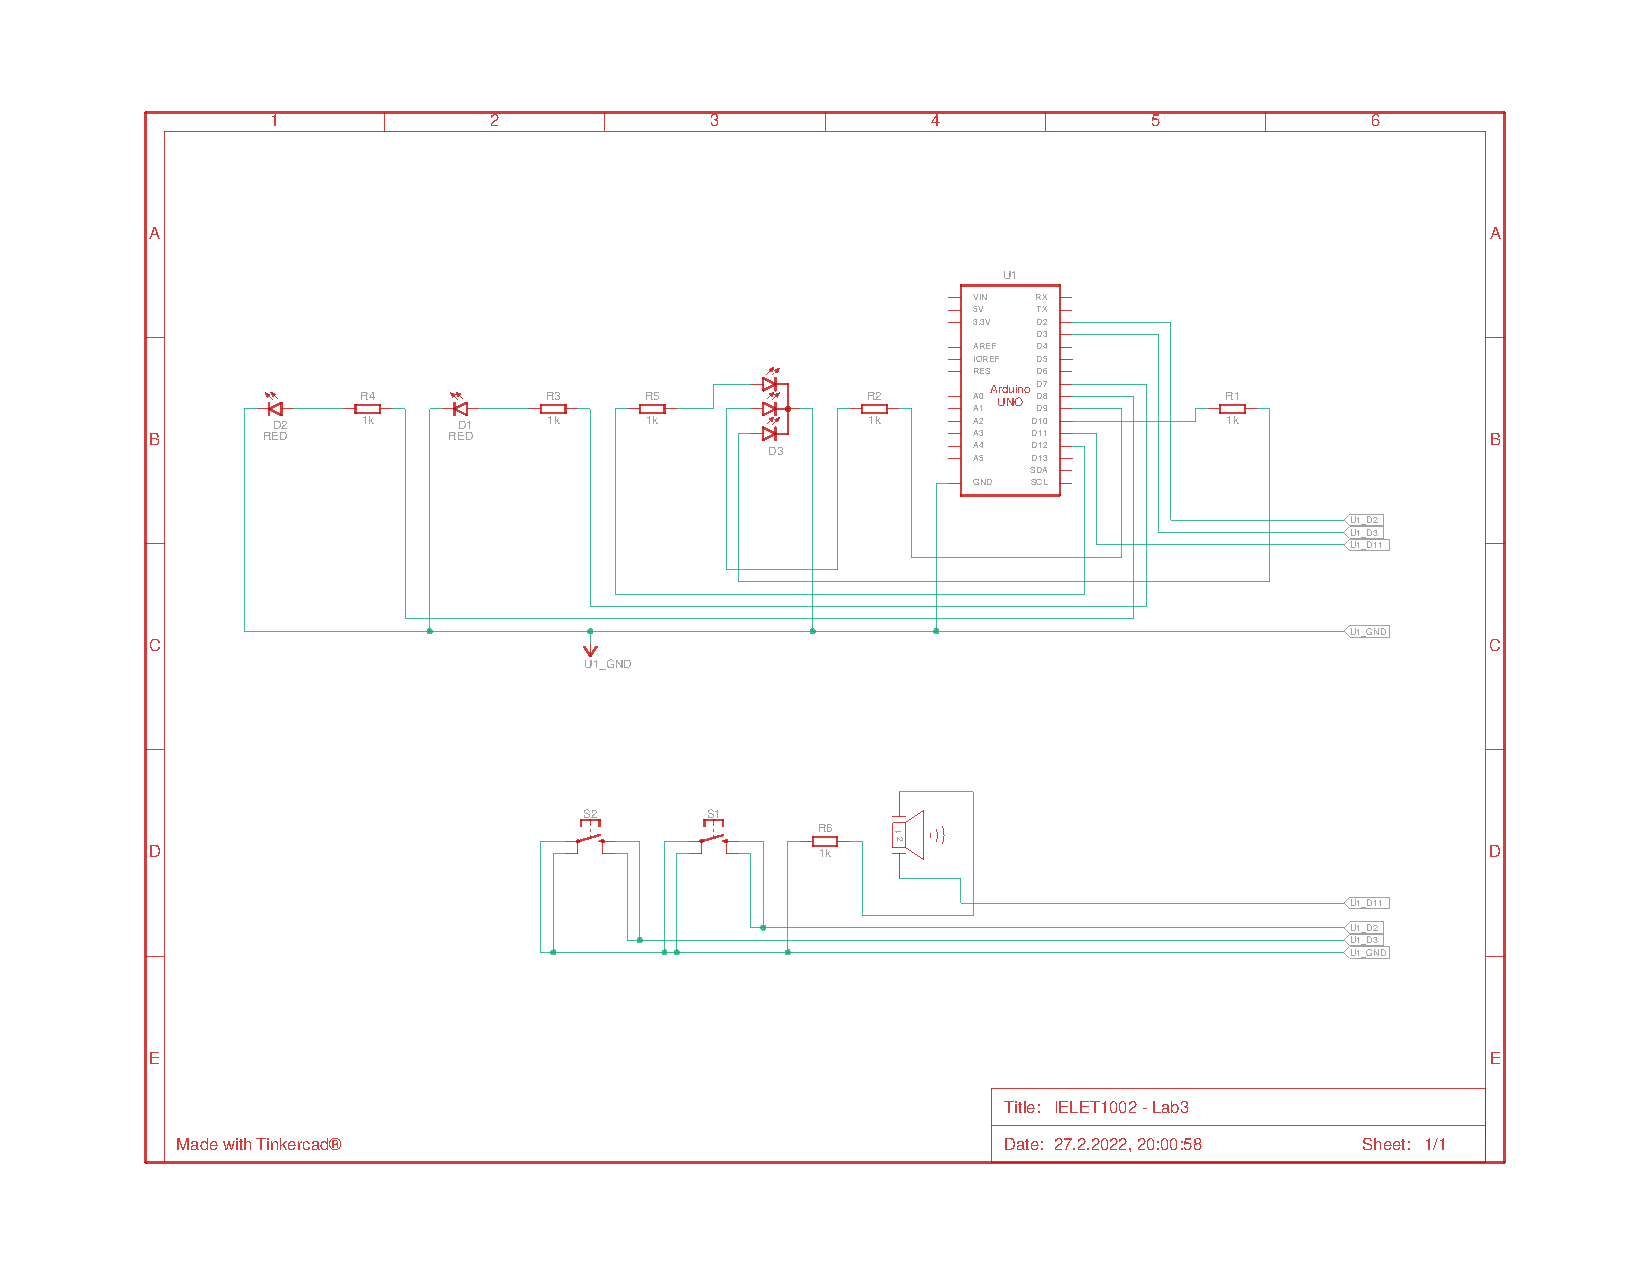
\includegraphics[width=0.53\textwidth, trim={0 2cm 0 2cm}]{images/wiring-diagram.pdf}
    \caption{Wiring Diagram}
    \label{fig:wiring}
    \end {center}
\end{figure}

\vfill\null
\pagebreak

\begin{figure}[H]
    \begin {center}
    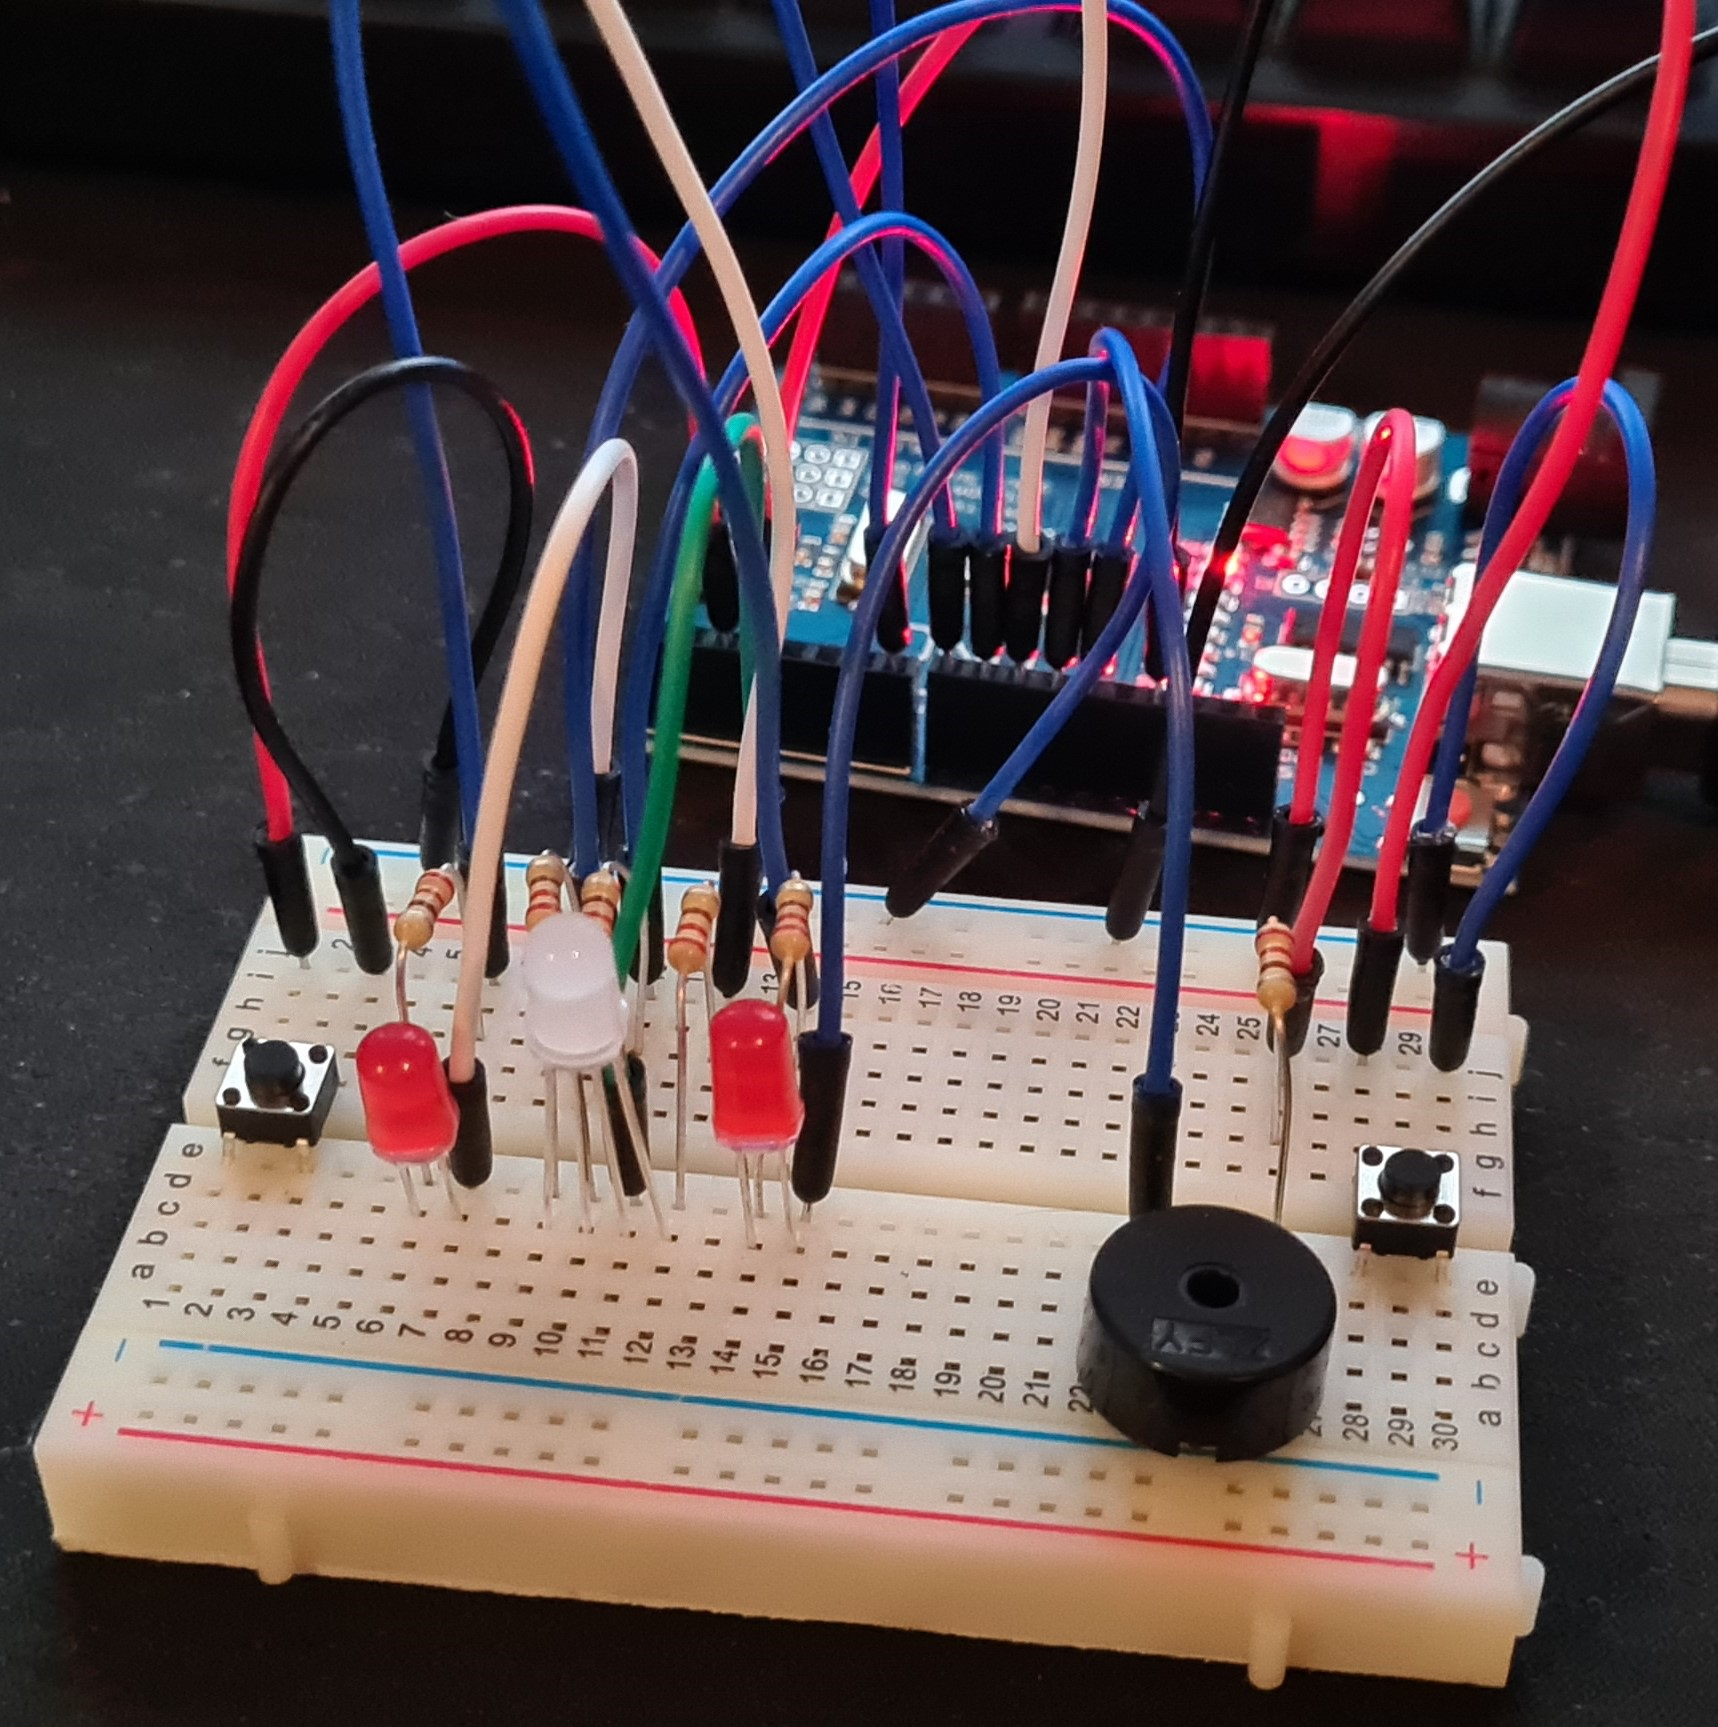
\includegraphics[width=0.45\textwidth]{images/circuit-picture.jpg}
    \caption{Lab3 Circuit}
    \label{fig:circuitPicture}
    \end {center}
\end{figure}

\begin{figure}[H]%[!ht]
    \begin {center}
    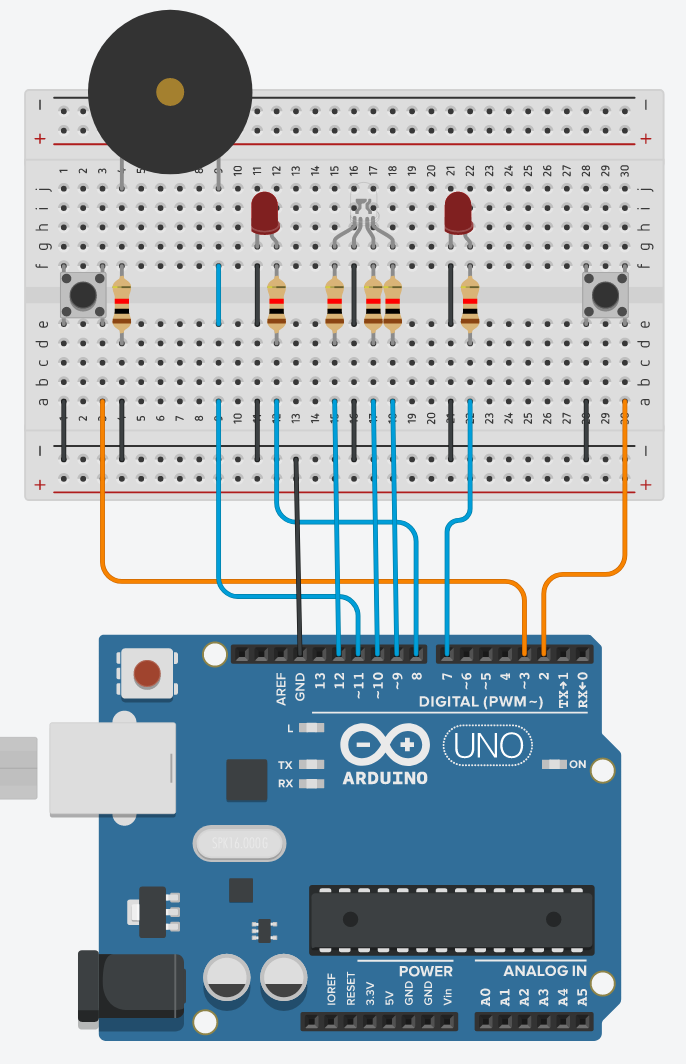
\includegraphics[width=0.45\textwidth]{images/tinkercad.PNG}
    \caption{Tinkercad}
    \label{fig:tinkercad}
    \end {center}
\end{figure}

\onecolumn

\subsection{Software}
Lets start by creating some configs to keep our code free of "magic constants".
By keeping these configs in separate files, we avoid cluttering our logic in the main.cpp file.\\


\lstinputlisting[language=C++, caption=Range.h]{../lib/Range/Range.h}
\lstinputlisting[language=C++, caption=PlayerConfig.h]{../lib/PlayerConfig/PlayerConfig.h}
\lstinputlisting[language=C++, caption=RgbLedConfig.h]{../lib/RgbLedConfig/RgbLedConfig.h}

\lstinputlisting[language=C++, caption=ApplicationConfig.h]{../lib/ApplicationConfig/ApplicationConfig.h}
This gives us a global const appConfig when we include the ApplicationConfig.h file
in our main sketch.

\vfill\null
\pagebreak

\lstinputlisting[language=C++, caption=Timer.h]{../lib/Timer/Timer.h}
We also create a Timer class to make time tracking a bit easier and more intuitive.

\vfill\null
\pagebreak

% main.cpp sections:

% imports
% Player
% RgbLed
% SerialCommand
% GameState
% ApplicationState
% SerialMessages
% Reset
% getBestPlayerIndex
% updateGameState
% fancySoundFunction
% printPoints
% indicateWinner
% indicateLooser
% waitForButtonsToBeUnpressed
% startGame
% setup
% loop


Now that all our external files are set up, we can start looking at the main.cpp file.
%https://stackoverflow.com/questions/3915709/latex-lstlisting-automatically-recognizing-code-passage
\lstinputlisting[language=C++, caption=main.cpp - imports, linerange=imports-End_Section]{../src/main.cpp}
We start by importing our external files and libraries.

\lstinputlisting[language=C++, caption=main.cpp - Player           , linerange=Player-End_Section]{../src/main.cpp}
Next we create a Player class that can keep track of its score, and put
all information about that player in one place. This also lets us create a
cleaner setup function with less room for error.

\vfill\null
\pagebreak

\lstinputlisting[language=C++, caption=main.cpp - RgbLed      , linerange=RgbLed-End_Section]{../src/main.cpp}
Properly managing the RGB LED turned in to a mess, and therefore i created helper functions
to ensure that the correct state was always set. This however turned in to a number of functions,
and for this reason i decided to create a RgbLed class. This also has a setup function like the Player class.

\lstinputlisting[language=C++, caption=main.cpp - SerialCommand      , linerange=SerialCommand-End_Section]{../src/main.cpp}
We create an enum of comments that the user may send to the arduino through the serial port.

\lstinputlisting[language=C++, caption=main.cpp - GameState      , linerange=GameState-End_Section]{../src/main.cpp}
We also create an enum for the GameState, that the serial commands will change.

\vfill\null
\pagebreak

\lstinputlisting[language=C++, caption=main.cpp - ApplicationState      , linerange=ApplicationState-End_Section]{../src/main.cpp}
Now that our datatypes are specified, we can create our ApplicationState struct, to keep
track of the mutable state in our game. We put the players in an array to make
manipulation of multiple players easier throughout the code, as well as making it easier to
expand the game to more players in the future.

\lstinputlisting[language=C++, caption=main.cpp - SerialMessages     , linerange=SerialMessages-End_Section]{../src/main.cpp}
Because we require Serial input to control the game, we should also provide
some feedback to the Serial port. To make this cleaner and reusable
in the code, we define functions for doing this.

\vfill\null
\pagebreak

\lstinputlisting[language=C++, caption=main.cpp - Reset     , linerange=Reset-End_Section]{../src/main.cpp}
Due to the sequential nature of this program, it is beneficial to create a function for
turning off IO that should be disabled after a section is done executing. By giving each
part of the program a clean slate, we can focus on only the IO that we care about.
We also create a function for resetting the game and player points.\\

Take notice that the for-loop uses the \& sybmol next to the player variable. This means
that the player variable is a reference to the actual player object.
C++ is by default "pass by value", meaning that if we were to remove the \& symbol,
a copy of the player at a given iteration would be assigned to the variable.
This has a clear performance issue, but more importantly it creates a rather interesting bug.
In this for-loop we alter the players internal point value. If this is a reference however,
only the internal point value of the copy will change, while the original player
object stored in the array will remain unchanged. This was likely the most noteworthy discovery
during this lab, and a rather fun issue to debug.

\lstinputlisting[language=C++, caption=main.cpp - getBestPlayerIndex     , linerange=getBestPlayerIndex-End_Section]{../src/main.cpp}
Because we have choosen to put the players in an array, we require a bit of logic to find the
best player from the list. Because of readability and the fact that we will need this logic
in several places of the program, we will create a function to do this.

\vfill\null
\pagebreak

\lstinputlisting[language=C++, caption=main.cpp - updateGameState     , linerange=updateGameState-End_Section]{../src/main.cpp}
Because the GameState can be changed at a whim by the serial commands, we need some constantly
running checks to make sure that the buzzer for example does not keep ringing after the
game is stopped. We also want to constantly check for user input. This logic
makes sense to put into its own function, to be run in all of our sequential while-loops.\\

Take notice that the code under the SerialCommand::STOP case is wrapped in curly braces.
This is because we needed to create a variable scoped only to that case. If we didn't add
the curly braces, the variable would be scoped to the entire function, and because that
would mean a conditional decleration inside the same scope, it would be a syntax error.

\lstinputlisting[language=C++, caption=main.cpp - fancySoundFunction     , linerange=fancySoundFunction-End_Section]{../src/main.cpp}
To make the game more interesting, we want the winner sound to be something other than a simple
linear ramp. To do this, we jump into GeoGebra and select an arbitrary mathematical expression
to modulate the buzzer tone. The code vaguely represents this graph:

\begin{figure}[H]%[!ht]
    \begin {center}
    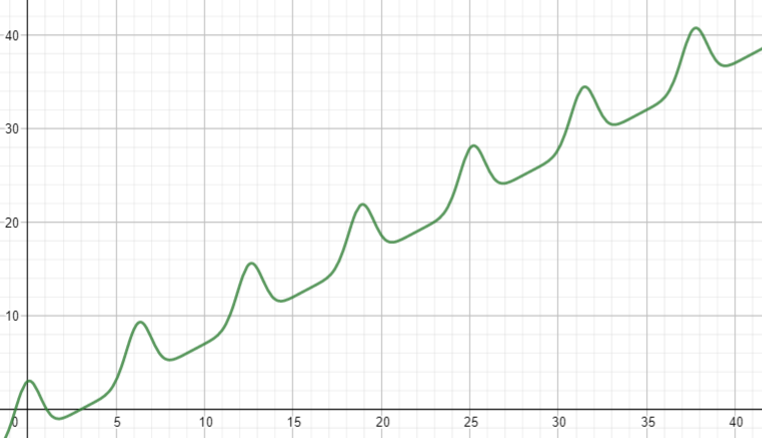
\includegraphics[width=\textwidth]{images/sound-function.PNG}
    \caption{Sound Function}
    \label{fig:sound-function}
    \end {center}
\end{figure}

\lstinputlisting[language=C++, caption=main.cpp - printPoints     , linerange=printPoints-End_Section]{../src/main.cpp}
Before we implement the logic for celebrating the winner and mocking the looser, we create a function to print
the current score of all players to the serial port.

\lstinputlisting[language=C++, caption=main.cpp - indicateWinner     , linerange=indicateWinner-End_Section]{../src/main.cpp}
Because the exercise requires the use of a for-loop, we have a loop-hole \(pun intended\). A for loop has 3 sections
where the middle one is an evaluation. If we leave the two first empty, we get the same effect as a while-loop.
Notice the use of the blinkTimer. It allows us to make the led blink, without using delay\(\). This way we
can not only implement fancy audio such as depicted above, but also have a very low responsetime when user input
is detected from the serial port.

\lstinputlisting[language=C++, caption=main.cpp - indicateLooser     , linerange=indicateLooser-End_Section]{../src/main.cpp}
Notice that because we are not waiting for a RAMP in this function, we need an additional timer. This
is easy and clean to implement however, because we created our Timer class.

\lstinputlisting[language=C++, caption=main.cpp - waitForButtonsToBeUnpressed     , linerange=waitForButtonsToBeUnpressed-End_Section]{../src/main.cpp}
Before we implement the game loop itself, we need one last helper function. This was the result of a
rather cumbersome debugging session. The ezButton library seems to behave strangely when a round ends,
and keeps reporting the button being pressed during the first update. Why? I don't know. Most likely
it has something to do with the debouncing, and frankly i had better things to do.
Without anything mentioned about it in the documentation, i decided to add a sanity check
before starting a new round of the game. Now, the game will not continue until all the buttons have
been released. The fix is rather simple, but such a solution should not be used in production code.

\lstinputlisting[language=C++, caption=main.cpp - startGame     , linerange=startGame-End_Section]{../src/main.cpp}
Finally we get to the startGame function, which is our game loop.
Here all of our choices pay off. From the use of three timers, the convenience of the updateGameState function,
the RGB LED logic as helper functions, and the players inserted into an array all make this code very readable.
Imagine if we had to manually disable the 3 other colors on the RGB in each branch, or write a separate function
that checked and updated each player as well as its button. With our current setup, this rather complex logic
has become easy to implement. Also note that the updateGameState\(\) logic is identical to indicateWinner
and indicateLooser. Consistency makes it easier for someone new to enter a codebase with which they are
unfemiliar.This is great if you are working in a team, or need to get back to your own code after some time.

\lstinputlisting[language=C++, caption=main.cpp - Setup              , linerange=setup-End_Section]{../src/main.cpp}
Now that we have completed our game loop, we will create the void setup\(\) function
Again we see the benefit of putting our players in an array. If we wish
to add more players in the future, we are not at risk of forgetting to
call setup for their IO, as the for-loop does not care about the number of
players involved.\\

At the end of the setup function, we also call printHelp\(\) to show an initial
set of instructions to the user.

\lstinputlisting[language=C++, caption=main.cpp - loop               , linerange=loop-End_Section]{../src/main.cpp}
And here we arrive at the last piece of code in the project. The main loop.
Because everythin has been defined in its own function, it is very clean and
easy to follow and expand upon.

\section{Discussion}
Because the solution i picked for this lab was very similar to lab2,
the same discussion applies:\\

The current code works excellently, however it does have a weakness.
While the nested nature of this code makes for very few instances of "state" and
globals, it does prevent us from running continous updates on anything while
a piece of code is executing. In a larger project, i believe it would be
beneficial to avoid while and for-loops, in favour of a more flat architecture with
state machines. That way, the project remains scalable, and we can easily add
continous checks without risking spagheti code and human errors due to forgetting
to call an updater during a special loop.\\

In this project this weakness becomes a real problem, as we had to create helpers
such as resetIo\(\) to keep our sanity. Perhaps the next lab will present a case
where the current solutions' drawbacks far outweigh its benefits, and a new
solution must be choosen to address them.

\vfill\null
\pagebreak

\section{Large Images}

\begin{figure}[h]
    \begin {center}
    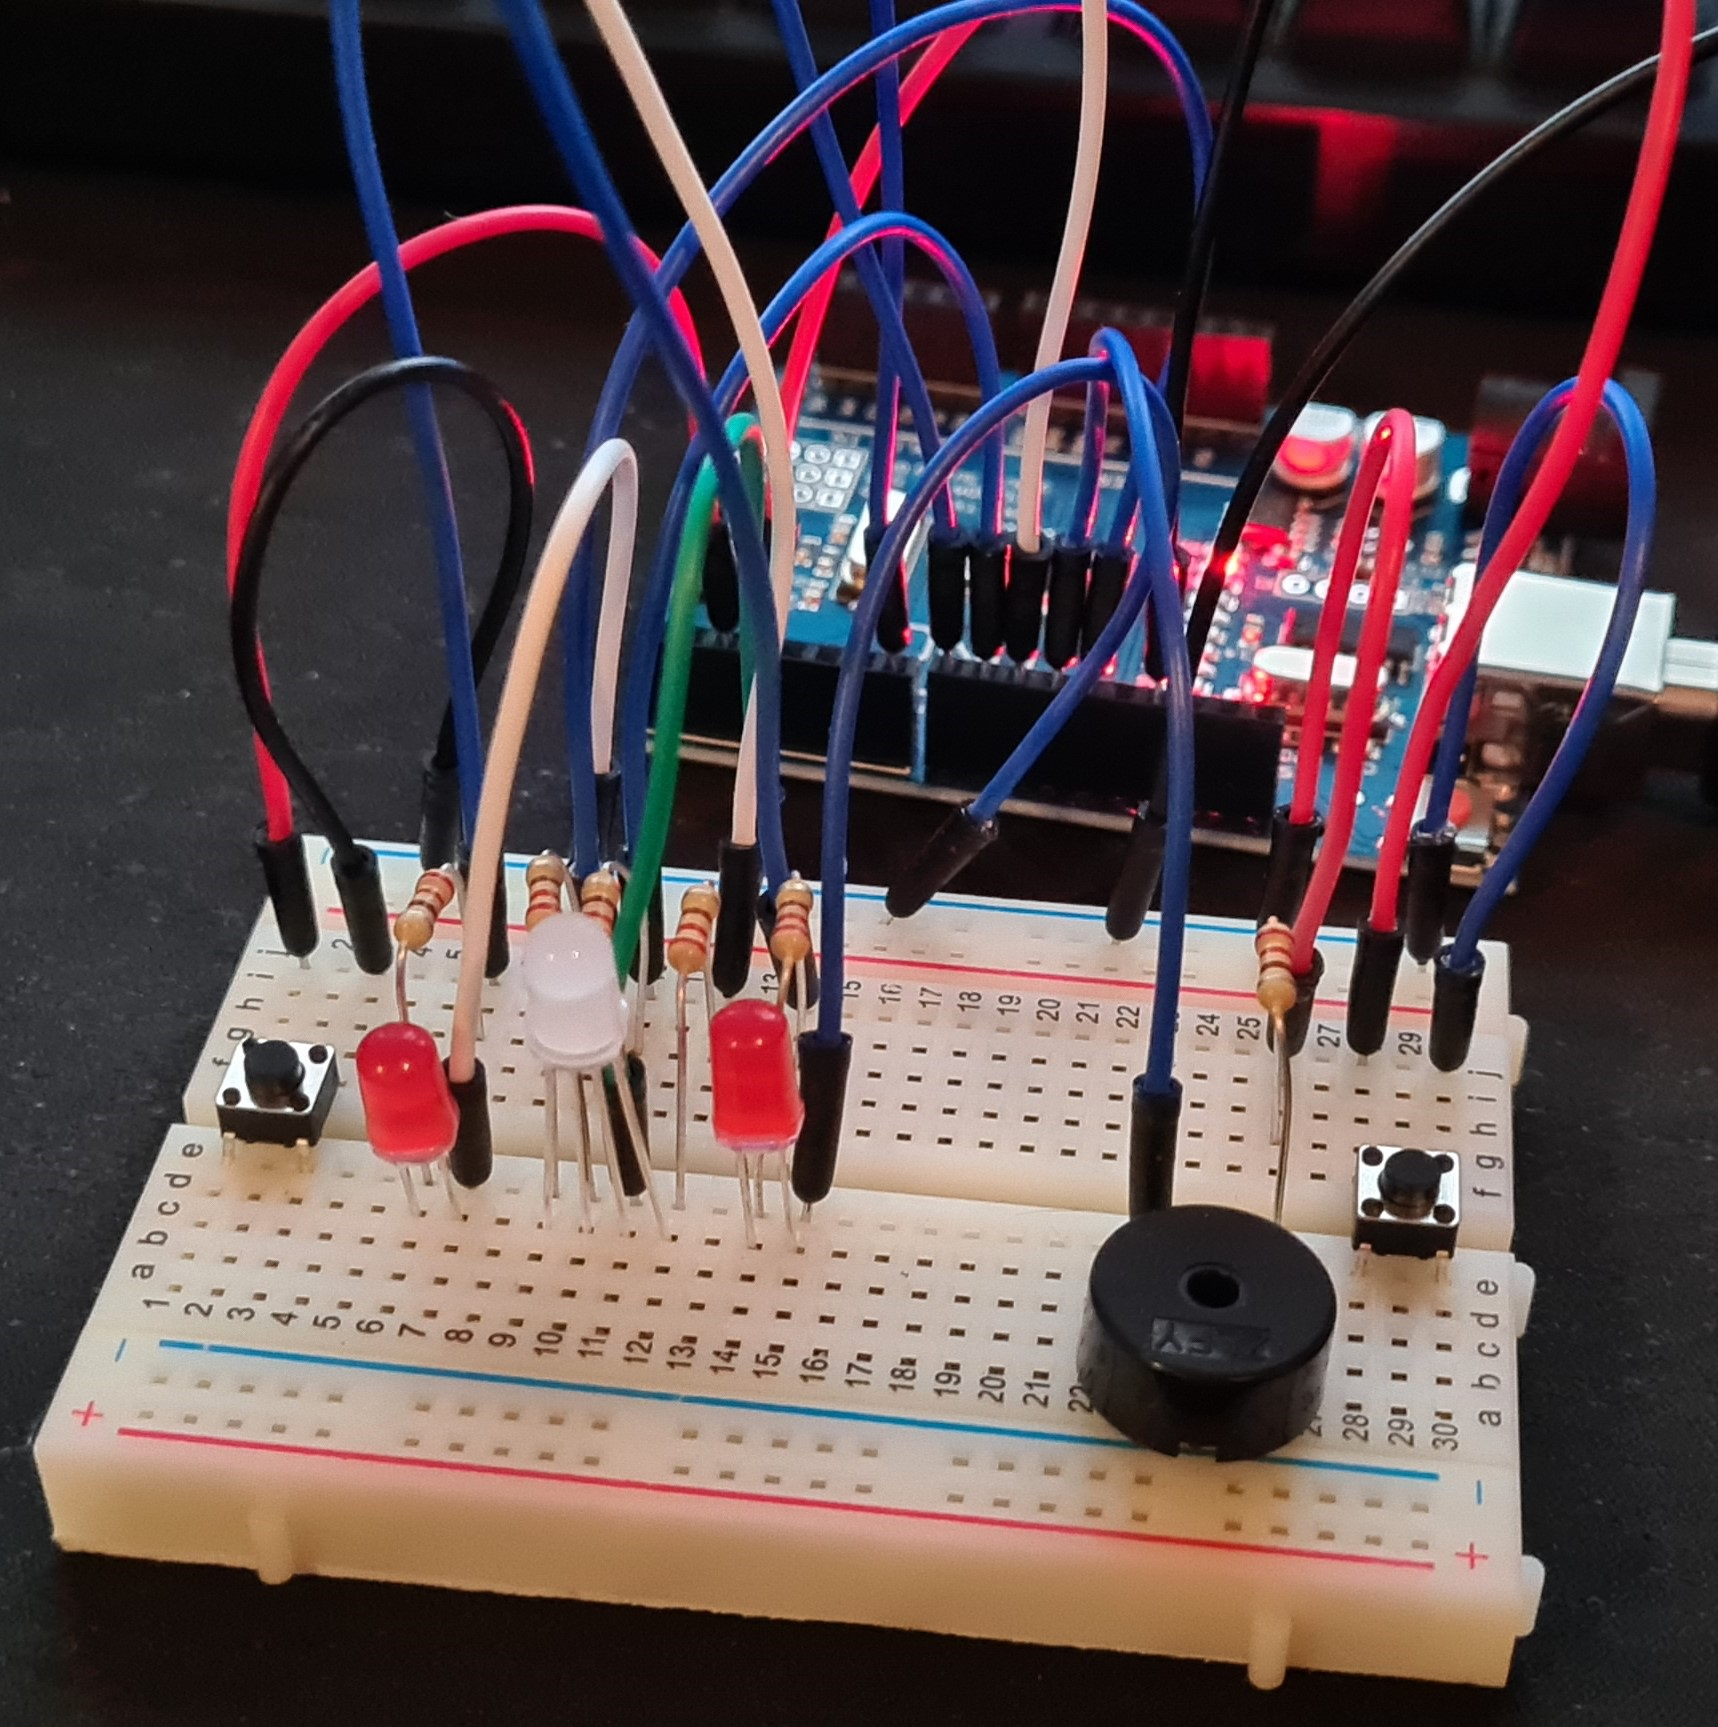
\includegraphics[width=\textwidth]{images/circuit-picture.jpg}
    \caption{Large Lab2 Circuit}
    \label{fig:circuitPictureLarge}
    \end {center}
\end{figure}

\begin{landscape}

    \begin{figure}[h]%[!ht]
        \begin {center}
        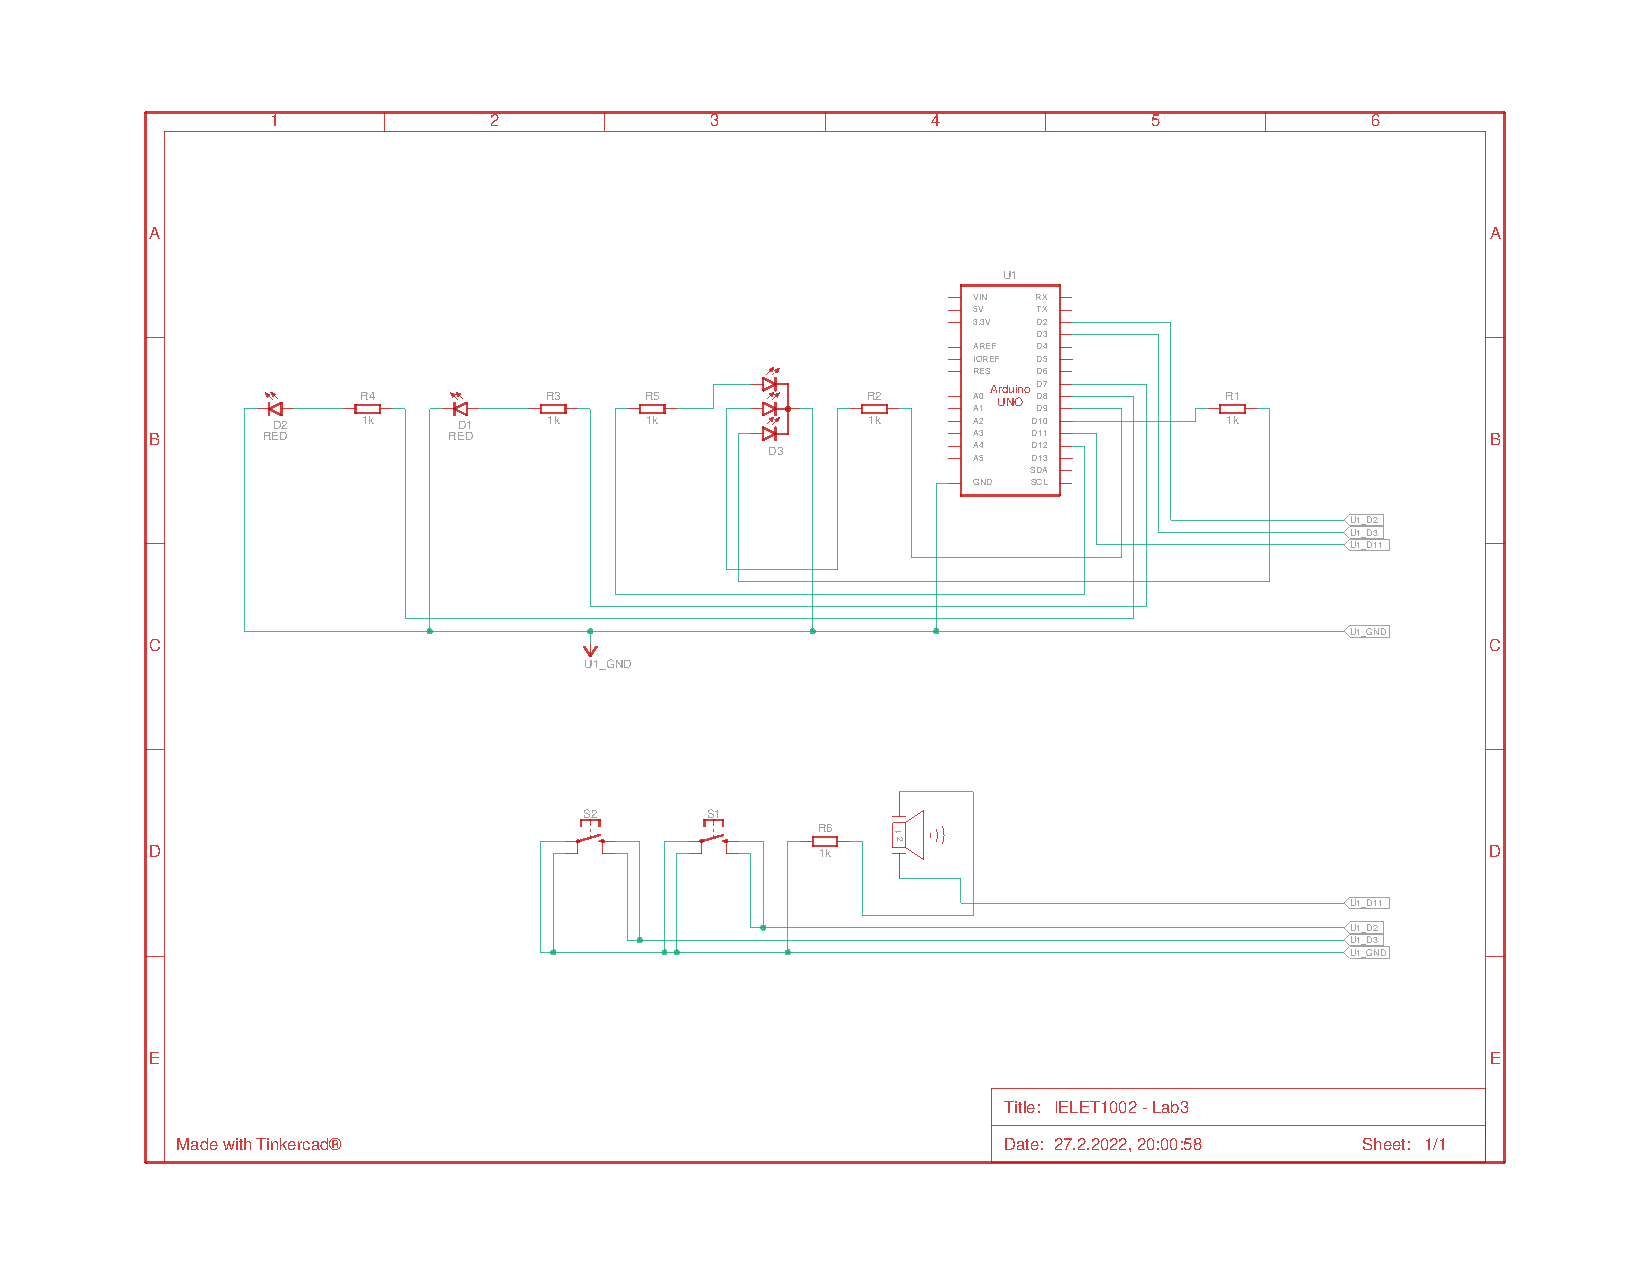
\includegraphics[width=1.5\textwidth, trim={0 2cm 0 2cm}]{images/wiring-diagram.pdf}
        \caption{Large Wiring Diagram}
        \label{fig:wiringLarge}
        \end {center}
    \end{figure}

    \begin{figure}[h]%[!ht]
        \begin {center}
        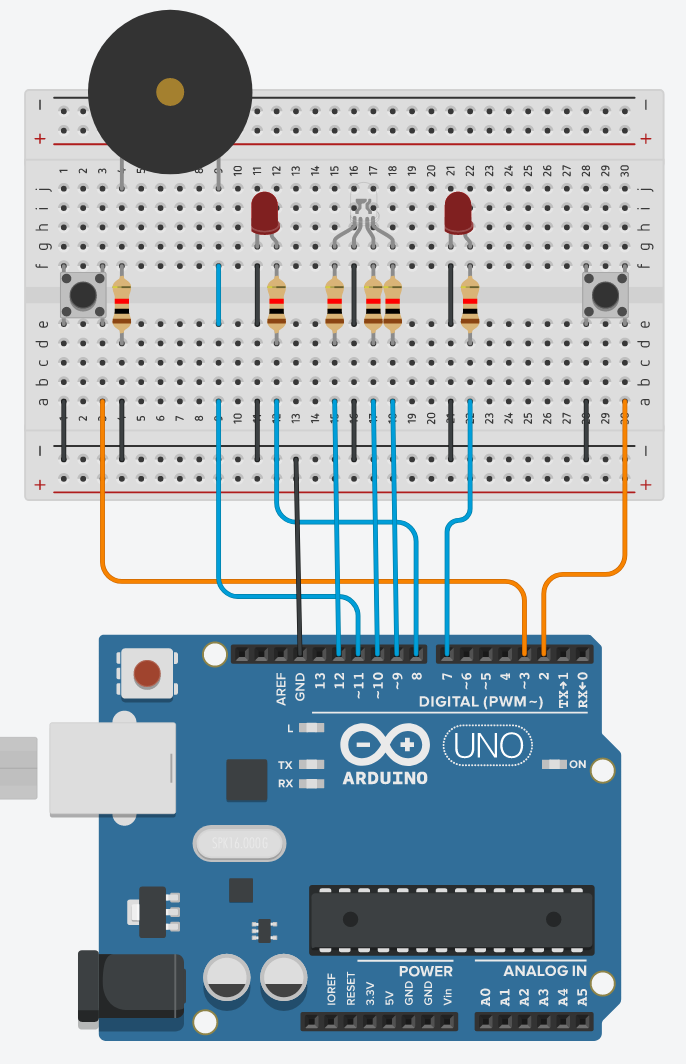
\includegraphics[width=\textwidth, angle=90]{images/tinkercad.PNG}
        \caption{Large Tinkercad}
        \label{fig:tinkercadLarge}
        \end {center}
    \end{figure}

\end{landscape}

\end{document}


